Important: Neighborhoods, FLip and swap?. Search methods RW, BI, and FI (sidewalks). Heuristics obj var only and 
conflicting var only. Meta heuristic, Tabu search (tabu tenure, aspiration, Search procedure FI or BI, Neighborhood 
limitations for large neighborhoods?). Combining search procedure. \boste{Make overview of classes and methods} \\ \\ 
Local search can 
be seen as a walk through the neighborhood graph \boste{Should be defined earlier} going from one sol

The \class{LocalSearchEngine} class uses the model created for local search described in section \ref{sec_ls} and 
uses local search to improve the initial solution. When talking about variables in this section, it only refers to 
independent variables unless otherwise stated. Pointers to the independent variables are kept in a standard vector, 
called mask, and is shuffled to give a random sequence.   \\ 
Local search explores how changing value of few variables will affect the solution quality, hence exploring a neighbor 
solution. The key for being efficient is to compute this evaluation fast and the dependency digraph and the propagation 
queues are used for this. For simplicity let us first consider the step involving changing the value of a single 
variable $x$. The change of variable value is send through the dependency digraph where each invariants, reachable from 
the vertex representing $x$, is updated. The propagation queue is used to determine the sequence the invariants should 
be updated. This will update invariants that represent violation of constraints with different priority and the 
evaluation function. \\
If a step consist of more variables changing values, such as swapping values of two variables, the propagation queues 
of these variables can be merged. The merging should remove duplicates and keep the invariants topological sorted. The 
invariants unique time stamp can be used to keep the ordering. The new queue gives an ordering the invariants should be 
updated such that they are only updated once during each step. \\ 
Before making a step several neighbor solution might be explored before choosing a neighbor solution by applying a 
neighborhood operation. To evaluate a neighborhood operation a delta value for each invariant is used. The delta value 
is the value an invariant would change if the neighborhood operation is performed. By this we can evaluate the neighbor 
solution without performing a step. \\ 
Each constraint $c \in C$ created in the model was given a priority $p$ and these priorities are used during local 
search and let $k$ denote the highest priority given. \boste{Define $V(c)$, violation degree and $P(c) > 0$ priority of 
c }. Let $q_p \in Q$ be the sum of violation degree $V(c)$ of constraints with priority $p$. The evaluation functions 
value is consider as $q_0$ and the vector $Q$ is used to evaluate the quality of a solution. Two candidate solutions 
$\tau$ and $\tau'$ each have a vector of quality $Q_\tau$ and $Q_{\tau'}$ respectively. To determine which of the two 
solution are best their vector can be compared, starting with position $k$ and going backwards. The first position they 
have different value determine which solution is best, the one with the lowest value. Illustrated with a small example: 
\\ 
\begin{align}
 Q_\tau &= (5,2,4,2) \\ 
 Q_{\tau'} &=(10,6,3,2) 
\end{align}
Violation degrees of constraints with priority 3 ($Q_\tau[3]$, $Q_{\tau'}[3]$) contributes with 2 in each candidate 
solution and then the violation degree of priority 2 is consider. Then candidate solution $\tau'$ is consider better 
than $\tau$ since $Q_\tau(2) = 4$ $>$ $Q_{\tau'}(2) = 3$. An invariant is created for each priority $p$ and one for the 
evaluation function before the local search begin at the same time invariants are created by each constraint class. \\
The new classes used for local search are in three different categorize, moves, neighborhoods, and search 
procedures. A \class{Move} object stores information of a neighborhood operation including the change of the evaluate 
function and change of violations. A subclass of the \class{Neighborhood} class is the choice of step function and 
gives the sequence the neighbor solutions are explored. They also determine how neighborhood operation are calculated 
and how steps are performed. The search procedures can quire a \class{Neighborhood} class to evaluate a 
neighborhood operations, a \class{Move}, effect on the evaluation function. It is the search procedures that determine 
which neighbor solution to go to if any. Neighborhoods and search procedures are combined to create different local 
search algorithms and \class{LocalSearchEngine} uses them within the time limit to improve the solution. \\ 
\begin{figure}[!b]
\begin{center}
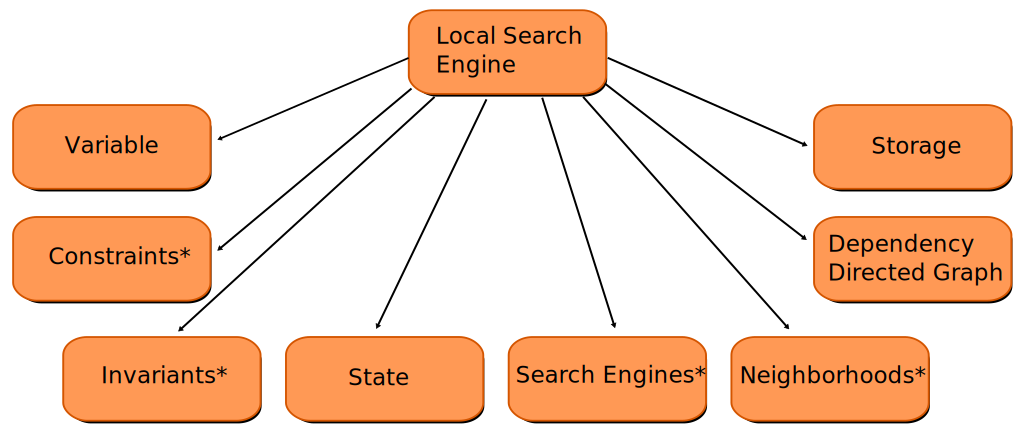
\includegraphics[width=0.9\linewidth]{LSE}\caption{Overview of the class pointers of Local Search Engine. The fields 
marked with a star (*) are several classes of that type.} 
\label{fig_lse}
\boste{Variable og constraint til venstre, think this should be posted earlier} 
\end{center}
\end{figure}
